\section{Theoretical Methodology}\label{Sec: Theoretical Methodology}

In this part, we elaborate on and enhance the algorithm proposed in \cite{scc_tree_reference}
for maintaining strongly connected components (SCCs) under a sequence of updates. 
The algorithm is designed to accommodate n vertices and m edges as input, proficiently manages the following operations:
\begin{itemize}
 \item  \textsc{Query}(u, v): Verifies whether both u and v belong to the same SCC.
 \item  \textsc{Delete}(u, v): Removes the edge from u to v.
\item  \textsc{Add}(u, v): Introduces the edge from u to v.
\end{itemize}

This algorithm achieves its objectives through the creation and continuous maintenance of a specialized data structure known as the SCC Tree, 
which is further explained in the subsequent section. 
Additionally, it employs an SCC mapping array to facilitate queries in constant time \textit{O(1)}.

The algorithm initiates with an initialization stage, wherein it constructs the proposed SCC tree 
and populates the SCC mapping array based on the identified strongly connected components within the graph. 
Subsequently, the process of constructing and maintaining these pivotal data structures under the delete and add updates is elaborated in the following sections, accompanied by their respective pseudo codes.

\subsection{Data Structures}\label{Subsec: Data Structures Theoretical}

In this section, we delve into a comprehensive exploration of the specialized data structures crucial to the functionality 
and efficiency of the algorithm. Through this detailed examination, we aim to provide clarity 
and insight into the design principles, operational mechanisms, and computational complexities of these structures.

\subsubsection{SCC Tree}\label{Subsubsec: SCC Tree}
The SCC tree serves as a vital component in maintaining the internal connectivity of vertices within the strongly connected components of graph G. 
For each SCC identified in the graph, a corresponding SCC tree is constructed.

The node in the SCC tree corresponding to the label $R$ encapsulates a tuple that can be represented as $\text{\textit{STN}}(R) = \lf( V, E \rt)$, 
where $V$ represents set of vertices and $E$ represents set of edges connecting them.
This encapsulation enables the SCC tree to maintain the connectivity of the vertices that are a part of the SCC labeled $R$,
also facilitating efficient traversal and update operations.

Each vertex $v \in V$ in the \ac{stn} of $R$ is a label uniquely associated with an SCC tree. 
This tree is a subtree of the SCC tree represented by the label $R$.
The SCC tree for a graph containing one vertex $v$ has only a single \ac{stn} represented as $\text{\textit{STN}}(v) = (\{v\}, \emptyset)$.

\begin{figure}[H]
    \centering
    \begin{subfigure}[b]{0.4\textwidth}
        \centering
        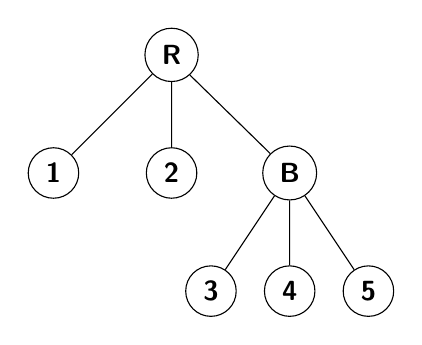
\begin{tikzpicture}[
            level distance=1.5cm,
            level 1/.style={sibling distance=1.5cm},
            level 2/.style={sibling distance=1cm},
            main node/.style={circle,draw,font=\sffamily\bfseries}]
                    % Define vertices
            \node[main node] (R) {R}
            child {node[main node] (1) {1}}
            child {node[main node] (2) {2}}
            child {node[main node] (B) {B}
                child {node[main node] (3) {3}}
                child {node[main node] (4) {4}}
                child {node[main node] (5) {5}}
            };
        \end{tikzpicture}
        \label{fig:example_scc_tree}
    \end{subfigure}
    \hfill
    \begin{subfigure}[b]{0.25\textwidth}
        \centering
        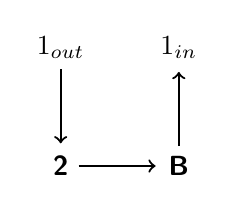
\begin{tikzpicture}[
            ->,shorten >=1pt,auto,node distance=1.5cm,
            thick,main node/.style={font=\sffamily\bfseries}]
            % Define vertices
        \node[main node] (1) {$1_{in}$};
        \node[main node] (11) [left of=1] {$1_{out}$};
        \node[main node] (2) [below of=11] {2};
        \node[main node] (B) [below of=1] {B};
        

        % Draw edges
        \path[every node/.style={font=\sffamily\small}]
            (11) edge (2)
            (2) edge (B)
            (B) edge (1);
        \end{tikzpicture}
        \caption{STN(R)}
        \label{fig:stn_r}
    \end{subfigure}
    \hfill 
    \begin{subfigure}[b]{0.25\textwidth}
        \centering
        \begin{tikzpicture}[
            ->,shorten >=1pt,auto,node distance=1.5cm,
            thick,main node/.style={font=\sffamily\bfseries}]
            % Define vertices
        \node[main node] (3) {$3_{in}$};
        \node[main node] (33) [left of=1] {$3_{out}$};
        \node[main node] (4) [below of=11] {4};
        \node[main node] (5) [below of=1] {5};
        

        % Draw edges
        \path[every node/.style={font=\sffamily\small}]
            (33) edge (4)
            (4) edge (5)
            (5) edge (3);
        \end{tikzpicture}
        \caption{STN(B)}
        \label{fig:stn_b}
    \end{subfigure}
    \caption{Example SCC Tree and its corresponding STNs}
    \label{fig:figure_with_subfigures}
\end{figure}

The SCC tree shown in \figureref{\ref{fig:figure_with_subfigures}}, can be represented by a collection of STNs as follows:
\begin{itemize}
    \item $\text{\textsc{STN}}(R)=(\{1,2,B\}, \{(1,2), (2,B), (B,1)\})$
    \item $\text{\textsc{STN}}(B)=(\{3,4,5\}, \{(3,4), (4,5), (5,3)\})$
    \item $\text{\textsc{STN}}(v)=\lf(\{v\}, \emptyset\rt) \forall v \in \{1,2,3,4,5\}$
\end{itemize}
The SCC tree represented by label $B$ contains the STNs of $\{B,3,4,5\}$, which form a subtree of the SCC tree represented by label $R$,
similarly, the SCC tree represented by labels $\{1,2\}$ also form $R$'s subtree.

\subsubsection{SCC Mapping Array}\label{Subsubsec: SCC Mapping Array}
In graph G, each vertex $v$ is inherently associated with a strongly connected component (SCC), denoted by its corresponding SCC label. 
The SCC mapping array effectively captures this relationship between vertices and their respective SCC labels.

Suppose vertex $v$ in graph $G$ belongs to the strongly connected component labeled as $R$.
 In that case, we express this association using the SCC mapping array notation as $\text{\textit{SM}}_{G}(v)=R$. 
 This signifies that vertex $v$ is mapped to the SCC labeled as $R$ within the context of the graph $G$.


\subsection{Definitions}\label{Subsec: Definitions Theoretical}
In this section, we establish key definitions that form the foundation of the algorithms presented subsequently. 
These definitions are instrumental in understanding the intricacies of the algorithms and their associated data structures.

\subsubsection{\textit{FIND\_SCC}(G)}
\subsubsection{\textit{CONDENSE}(G)}
\subsubsection{\textit{SPLIT}(G)}
\subsubsection{\textit{MERGE}(G)}
\subsubsection{\textit{UNREACHABLE}(G)}


% subsection of construction of scc tree
\subsection{Constructing SCC Tree}

We will look at the construction of the SCC tree for the graph shown in \figureref{\ref{fig:graph1}}.
We start by finding all the SCCs of the graph and then construct the SCC-Tree for each SCC in it.
In the process of finding all the SCCs, we would also fill the SCC mapping array. 
A special tree node \textsc{STN}(M), called the master node would preserve the connectivity of the SCCs (condesed form of the original graph).

\begin{algorithm}[H]
    \SetAlgoLined
    \KwData{G}
    \KwResult{SCC mapping, \textsc{SccTree}s, \textsc{STN}(M)}
    $SM_{G} = \emptyset, \textsc{SccTree} = \emptyset$\;
    $S = \textsc{FindSccs}(G)$\;
    $V_l = \emptyset, E_l = E(G)$\;
    \For {each $s \in S$} {
        $L_s = \textsc{Label}(s)$\;
        $G_s = G \cap s$\;
        $\textsc{SccTree}(L_s) = \textsc{MakeTree}(G_s, L_s)$\;
        \For {each $v \in s$} {
            $SM_{G}(v) = L_s$\;
        }
        $V_l = V \cup \{L_s\}$\;
        $E_l = E_l - \{e \in E(G_s)\}$\;
    }
    $\textsc{STN}(M) = (V_l, E_l)$\;
    \Return $SM_{G}, \textsc{SccTree}s, \textsc{STN}(M) = (V_l, E_l)$\;

    \caption{\textsc{ConstructDS}(G)}
\end{algorithm}

Suppose we have a strongly connected graph $G$, the SCC Tree for the graph is constructed as follows:
\begin{itemize}
    \item If $|V(G)| = 1$ and $v \in V(G)$, then the SCC tree is $SCC(v) = STN(v) = (\{v\}, \emptyset)$.
    \item If $|V(G)| > 1$ and $d \in V(G)$, then the root SCC tree node would contain the graph \textsc{Condense}(\textsc{Split}($G, d$)), 
    and for each SCC in the graph \textsc{Condense}(\textsc{Split}($G, d$)), we add its SCC-tree as a subtree of R, with 
    exception that we would add only one tree for vertex $d$ instead of $d_{in}$ and $d_{out}$.
\end{itemize}

%algorithm
\begin{algorithm}[H]
    \SetAlgoLined
    \KwData{G | G is strongly connected, L | label of the root node}
    \KwResult{\textsc{SccTree(L)}}
    $v = random(V(G))$\;
    $\textsc{SccTree}(L) = \emptyset$\;
    \If {$|V(G)| = 1$} {
        $\textsc{STN}(L) = (\{v\}, \emptyset)$\;
        $\textsc{SccTree}(L) = \textsc{STN}(L)$\;
        \Return \textsc{SccTree}(L)\;
    }
    $G' = \textsc{Split}(G, v)$\;
    $S = \textsc{FindSccs}(G')$\;
    \For {each $s \in S$ and $v_{in} \not \in s$} {
        $L_s = \textsc{Label}(s)$\;
        $G_s = G' \cap s$\;
        $\textsc{SccTree}(L_s) = \textsc{MakeTree}(G_s, L_s)$\;
        $\textsc{SccTree}(L) = \textsc{SccTree}(L) \cup \textsc{SccTree}(L_s)$\;
    }
    $\textsc{STN}(L) = \textsc{Condense}(G')$\;
    $\textsc{SccTree}(L) = \textsc{SccTree}(L) \cup \textsc{STN}(L)$\;
    \Return \textsc{SccTree}(L)\;

    \caption{\textsc{MakeTree(G, L)}}
\end{algorithm}

We can understand the algorithm by looking at the following figures.
In \figureref{\ref{fig:graph1_and_condensed_graph1}}, we have the graph $G$, which is strongly connected.
Its condensed form would contain a single node $R$. The SCC mapping array would map all the nodes to $R$ and the master node 
would contain the graph in \figureref{\ref{fig:condensed_graph1}}.
\begin{figure}[H]
    \centering
    \begin{subfigure}{0.45\textwidth}
        \centering
        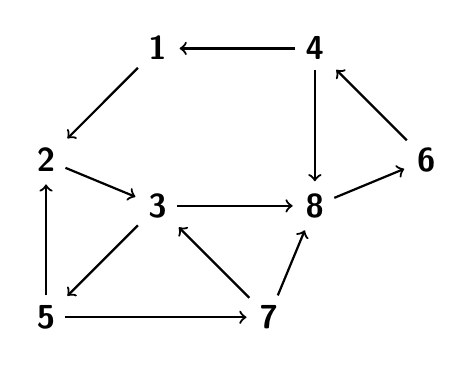
\begin{tikzpicture}[->,shorten >=1pt,auto,node distance=2cm,
            thick,main node/.style={font=\sffamily\large\bfseries}]

        % Define vertices
        \node[main node] (1) {1};
        \node[main node] (2) [below left of=1] {2};
        \node[main node] (3) [below of=1] {3};
        \node[main node] (4) [right of=1] {4};
        \node[main node] (5) [below left of=3] {5};
        \node[main node] (6) [below right of=4] {6};
        \node[main node] (7) [below right of=3] {7};
        \node[main node] (8) [right of=3] {8};
        

        % Draw edges
        \path[every node/.style={font=\sffamily\small}]
            (1) edge (2)
            (2) edge (3)
            (3) edge (5)
            (3) edge (8)
            (4) edge (1)
            (4) edge (8)
            (5) edge (2)
            (5) edge (7)
            (6) edge (4)
            (7) edge (3)
            (7) edge (8)
            (8) edge (6);

        \end{tikzpicture}
        \caption{Graph 1}
        \label{fig:graph1}
    \end{subfigure}
    \hfill
    \begin{subfigure}{0.45\textwidth}
        \centering
        
\begin{tikzpicture}[->,shorten >=1pt,auto,node distance=2cm,
            thick,main node/.style={circle,draw,font=\sffamily\bfseries}]

        % Define vertices
        \node[main node] (R) {R};

        \end{tikzpicture}
        \caption{condensed graph 1}
        \label{fig:condensed_graph1}
    \end{subfigure}
    \caption{Graph 1 and its condensed graph}
    \label{fig:graph1_and_condensed_graph1}
\end{figure}

After the strongly connected components of the graph are indentified, they are individually processed by the 
\textsc{MakeTree} algorithm. The algorithm starts by selecting a random vertex from the SCC and then splits the graph
on that vertex. The split graph is then condensed and the strongly connected components of the condensed graph are found. 
This is illustrated in \figureref{\ref{fig:scc_r_split_and_condensed_graph1}}, where we can see the condensed components $A$ and $B$.
The condesed graph in \figureref{\ref{fig:condensed_scc_r_split}} is stored in the \textsc{STN} of the root node $R$.
\begin{figure}[H]
    \centering
    \begin{subfigure}{0.45\textwidth}
        \centering
        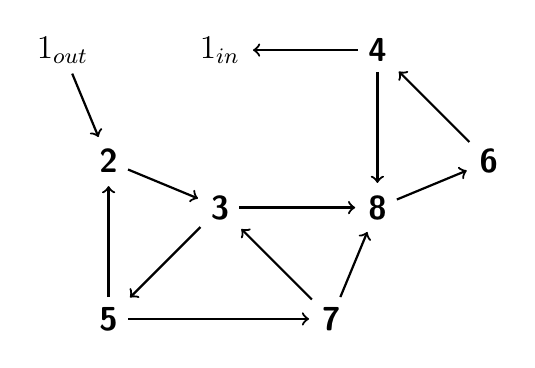
\begin{tikzpicture}[->,shorten >=1pt,auto,node distance=2cm,
            thick,main node/.style={font=\sffamily\large\bfseries}]

        % Define vertices
        \node[main node] (1) {$1_{in}$};
        \node[main node] (11) [left of=1] {$1_{out}$};
        \node[main node] (2) [below left of=1] {2};
        \node[main node] (3) [below of=1] {3};
        \node[main node] (4) [right of=1] {4};
        \node[main node] (5) [below left of=3] {5};
        \node[main node] (6) [below right of=4] {6};
        \node[main node] (7) [below right of=3] {7};
        \node[main node] (8) [right of=3] {8};
        

        % Draw edges
        \path[every node/.style={font=\sffamily\small}]
            (11) edge (2)
            (2) edge (3)
            (3) edge (5)
            (3) edge (8)
            (4) edge (1)
            (4) edge (8)
            (5) edge (2)
            (5) edge (7)
            (6) edge (4)
            (7) edge (3)
            (7) edge (8)
            (8) edge (6);

        \end{tikzpicture}
        \caption{SCC(R) split on 1}
        \label{fig:scc_r_split}
    \end{subfigure}
    \hfill
    \begin{subfigure}{0.45\textwidth}
        \centering
        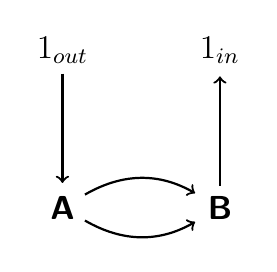
\begin{tikzpicture}[->,shorten >=1pt,auto,node distance=2cm,
            thick,main node/.style={font=\sffamily\large\bfseries}]

        % Define vertices
        \node[main node] (1) {$1_{in}$};
        \node[main node] (11) [left of=1] {$1_{out}$};
        \node[main node] (A) [below of=11] {A};
        \node[main node] (B) [below of=1] {B};
        

        % Draw edges
        \path[every node/.style={font=\sffamily\small}]
            (11) edge (A)
            (A) edge[bend left] (B)
            (A) edge[bend right] (B)
            (B) edge (1);

        \end{tikzpicture}
        \caption{condensed graph}
        \label{fig:condensed_scc_r_split}
    \end{subfigure}
    \caption{SCC(R) split on 1 and its condensed graph}
    \label{fig:scc_r_split_and_condensed_graph1}
\end{figure}

The \textsc{MakeTree} algorithm then processes all the condensed components of the split graph in a recursive manner.
The condensed component $A$ is split on 2, as in \figureref{\ref{fig:scc_a_split_and_condensed_graph1}}, and the 
condensed component $B$ is split on 4, as shown in \figureref{\ref{fig:scc_b_split_and_condensed_graph1}}. The 
component $A$ contains $C$ which is split on 3, as shown in \figureref{\ref{fig:scc_c_split_and_condensed_graph1}}.
The condesed graphs in \figureref{\ref{fig:condensed_scc_a_split}}, \figureref{\ref{fig:condensed_scc_b_split}}, and
\figureref{\ref{fig:condensed_scc_c_split}} are stored in the \textsc{STN} of $A$, $B$, and $C$ respectively.
\begin{figure}[H]
    \centering
    \begin{subfigure}{0.45\textwidth}
        \centering
        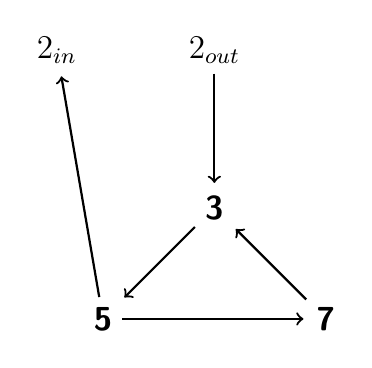
\begin{tikzpicture}[->,shorten >=1pt,auto,node distance=2cm,
            thick,main node/.style={font=\sffamily\large\bfseries}]

        % Define vertices
        \node[main node] (2) {$2_{out}$};
        \node[main node] (22) [left of=2] {$2_{in}$};
        \node[main node] (3) [below of=2] {3};
        \node[main node] (5) [below left of=3] {5};
        \node[main node] (7) [below right of=3] {7};
        

        % Draw edges
        \path[every node/.style={font=\sffamily\small}]
            (2) edge (3)
            (3) edge (5)
            (5) edge (22)
            (5) edge (7)
            (7) edge (3);

        \end{tikzpicture}
        \caption{SCC(A) split on 2}
        \label{fig:scc_a_split}
    \end{subfigure}
    \hfill
    \begin{subfigure}{0.45\textwidth}
        \centering
        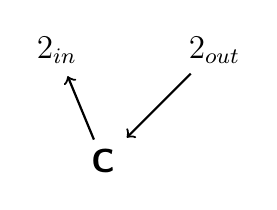
\begin{tikzpicture}[->,shorten >=1pt,auto,node distance=2cm,
            thick,main node/.style={font=\sffamily\large\bfseries}]

        % Define vertices
        \node[main node] (2) {$2_{out}$};
        \node[main node] (22) [left of=2] {$2_{in}$};
        \node[main node] (C) [below left of=2] {C};
        

        % Draw edges
        \path[every node/.style={font=\sffamily\small}]
            (2) edge (C)
            (C) edge (22);

        \end{tikzpicture}
        \caption{condensed graph}
        \label{fig:condensed_scc_a_split}
    \end{subfigure}
    \caption{SCC(A) split on 2 and its condensed graph}
    \label{fig:scc_a_split_and_condensed_graph1}
\end{figure}

\begin{figure}[H]
    \centering
    \begin{subfigure}{0.45\textwidth}
        \centering
        \begin{tikzpicture}[->,shorten >=1pt,auto,node distance=2cm,
            thick,main node/.style={font=\sffamily\large\bfseries}]

        % Define vertices
        \node[main node] (4) {$4_{in}$};
        \node[main node] (44) [left of=1] {$4_{out}$};
        \node[main node] (6) [below of=1] {6};
        \node[main node] (8) [below of=11] {8};
        

        % Draw edges
        \path[every node/.style={font=\sffamily\small}]
            (44) edge (8)
            (8) edge (6)
            (6) edge (4);

        \end{tikzpicture}
        \caption{SCC(B) split on 4}
        \label{fig:scc_b_split}
    \end{subfigure}
    \hfill
    \begin{subfigure}{0.45\textwidth}
        \centering
        \begin{tikzpicture}[->,shorten >=1pt,auto,node distance=2cm,
            thick,main node/.style={font=\sffamily\large\bfseries}]

        % Define vertices
        \node[main node] (4) {$4_{in}$};
        \node[main node] (44) [left of=1] {$4_{out}$};
        \node[main node] (6) [below of=1] {6};
        \node[main node] (8) [below of=11] {8};
        

        % Draw edges
        \path[every node/.style={font=\sffamily\small}]
            (44) edge (8)
            (8) edge (6)
            (6) edge (4);

        \end{tikzpicture}
        \caption{condensed graph}
        \label{fig:condensed_scc_b_split}
    \end{subfigure}
    \caption{SCC(B) split on 4 and its condensed graph}
    \label{fig:scc_b_split_and_condensed_graph1}
\end{figure}

\begin{figure}[H]
    \centering
    \begin{subfigure}{0.45\textwidth}
        \centering
        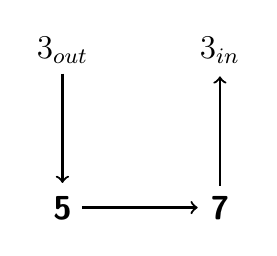
\begin{tikzpicture}[->,shorten >=1pt,auto,node distance=2cm,
            thick,main node/.style={font=\sffamily\large\bfseries}]

        % Define vertices
        \node[main node] (3) {$3_{in}$};
        \node[main node] (33) [left of=3] {$3_{out}$};
        \node[main node] (5) [below of=33] {5};
        \node[main node] (7) [below of=3] {7};
        

        % Draw edges
        \path[every node/.style={font=\sffamily\small}]
            (33) edge (5)
            (5) edge (7)
            (7) edge (3);

        \end{tikzpicture}
        \caption{SCC(C) split on 3}
        \label{fig:scc_c_split}
    \end{subfigure}
    \hfill
    \begin{subfigure}{0.45\textwidth}
        \centering
        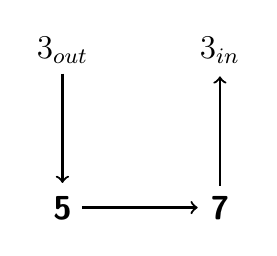
\begin{tikzpicture}[->,shorten >=1pt,auto,node distance=2cm,
            thick,main node/.style={font=\sffamily\large\bfseries}]

        % Define vertices
        \node[main node] (3) {$3_{in}$};
        \node[main node] (33) [left of=3] {$3_{out}$};
        \node[main node] (5) [below of=33] {5};
        \node[main node] (7) [below of=3] {7};
        

        % Draw edges
        \path[every node/.style={font=\sffamily\small}]
            (33) edge (5)
            (5) edge (7)
            (7) edge (3);

        \end{tikzpicture}
        \caption{condensed graph}
        \label{fig:condensed_scc_c_split}
    \end{subfigure}
    \caption{SCC(C) split on 3 and its condensed graph}
    \label{fig:scc_c_split_and_condensed_graph1}
\end{figure}

The figure \figureref{\ref{fig:scc_tree_graph1}} shows the SCC tree for the graph in \figureref{\ref{fig:graph1}}.
The SCC tree is constructed by the \textsc{MakeTree} algorithm, which recursively processes the condensed components of the split graph.
The child of each parent node in the SCC tree is a node present in the \textsc{STN} of the parent node.
\\$\textsc{SccTree(R)} = \textsc{STN}\text{'s of } \{R, 1, A, 2, C, 3, 5, 7, B, 4, 6, 8\}$


\begin{figure}[H]
    \centering
    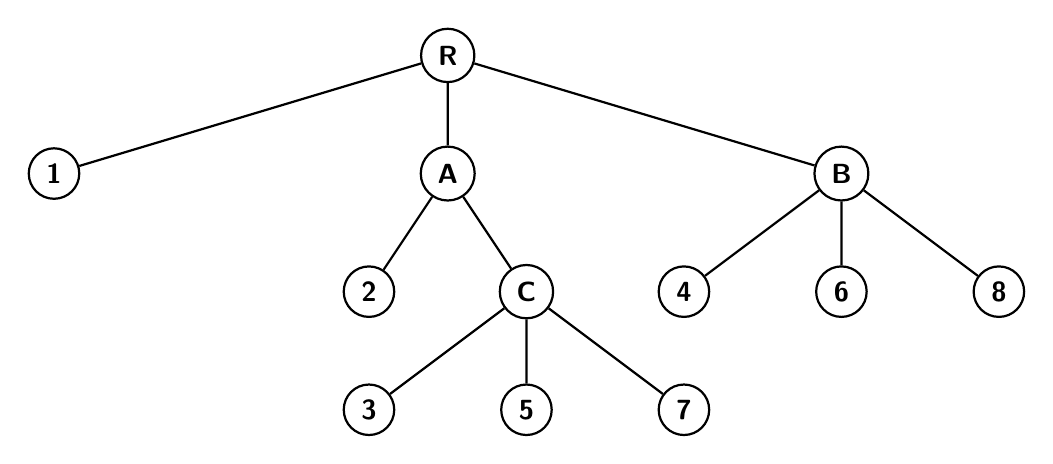
\begin{tikzpicture}[level distance=1.5cm,
                        level 1/.style={sibling distance=5cm},
                        level 2/.style={sibling distance=2cm},
                        thick,main node/.style={circle,draw,font=\sffamily\bfseries}]

      % Define vertices
      \node[main node] (R) {R}
        child {node[main node] (1) {1}}
        child {node[main node] (A) {A}
          child {node[main node] (2) {2}}
          child {node[main node] (C) {C}
            child {node[main node] (3) {3}}
            child {node[main node] (5) {5}}
            child {node[main node] (7) {7}}
          }
        }
        child {node[main node] (B) {B}
          child {node[main node] (4) {4}}
          child {node[main node] (6) {6}}
          child {node[main node] (8) {8}}
        };

    \end{tikzpicture}
    \caption{SCC Tree of Graph \ref{fig:graph1}}
    \label{fig:scc_tree_graph1}
\end{figure}



\subsection{Decremental Maintaince of SCC Tree}\label{Subsec: Decremental Maintaince of SCC Tree}

\subsubsection{Deleting Edge from the Root Node}\label{Subsubsec: Deleting Edge from the Root Node}

\begin{figure}[H]
    \centering
    \begin{subfigure}{0.45\textwidth}
        \centering
        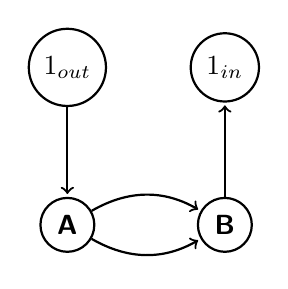
\begin{tikzpicture}[->,shorten >=1pt,auto,node distance=2cm,
            thick,main node/.style={circle,draw,font=\sffamily\bfseries}]

        % Define vertices
        \node[main node] (1) {$1_{in}$};
        \node[main node] (11) [left of=1] {$1_{out}$};
        \node[main node] (A) [below of=11] {A};
        \node[main node] (B) [below of=1] {B};
        

        % Draw edges
        \path[every node/.style={font=\sffamily\small}]
            (11) edge (A)
            (A) edge[bend left] (B)
            (A) edge[bend right] (B)
            (B) edge (1);

        \end{tikzpicture}
        \caption{Graph in SCC Tree Node R}
        \label{fig:tree_node_r_graph}
    \end{subfigure}
    \hfill
    \begin{subfigure}{0.45\textwidth}
        \centering
        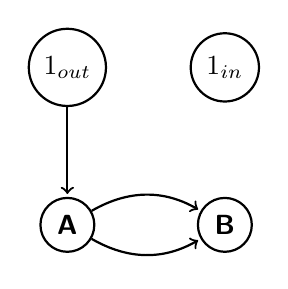
\begin{tikzpicture}[->,shorten >=1pt,auto,node distance=2cm,
            thick,main node/.style={circle,draw,font=\sffamily\bfseries}]

        % Define vertices
        \node[main node] (1) {$1_{in}$};
        \node[main node] (11) [left of=1] {$1_{out}$};
        \node[main node] (A) [below of=11] {A};
        \node[main node] (B) [below of=1] {B};
        

        % Draw edges
        \path[every node/.style={font=\sffamily\small}]
            (11) edge (A)
            (A) edge[bend left] (B)
            (A) edge[bend right] (B);

        \end{tikzpicture}
        \caption{Graph after deleting edge 4 to 1}
        \label{fig:graph_after_dedge_4_to_1}
    \end{subfigure}
    \caption{Graph in SCC Tree Node R after deleting edge 4 to 1}
    \label{fig:tree_node_r_graph_after_dedge1}
\end{figure}


\begin{figure}[H]
    \centering
    \begin{subfigure}{0.45\textwidth}
        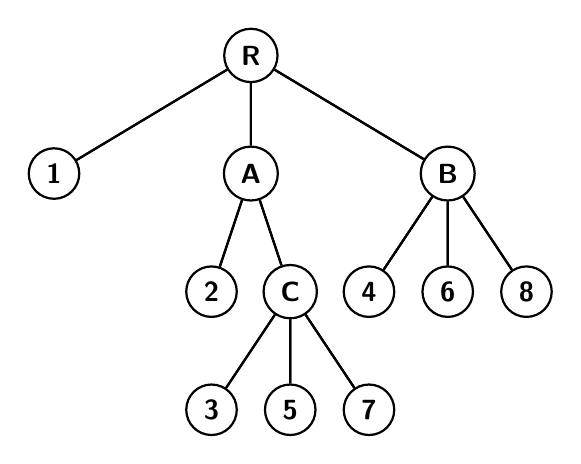
\begin{tikzpicture}[level distance=1.5cm,
                            level 1/.style={sibling distance=2.5cm},
                            level 2/.style={sibling distance=1cm},
                            thick,main node/.style={circle,draw,font=\sffamily\bfseries}]

        % Define vertices
        \node[main node] (R) {R}
            child {node[main node] (1) {1}}
            child {node[main node] (A) {A}
            child {node[main node] (2) {2}}
            child {node[main node] (C) {C}
                child {node[main node] (3) {3}}
                child {node[main node] (5) {5}}
                child {node[main node] (7) {7}}
            }
            }
            child {node[main node] (B) {B}
            child {node[main node] (4) {4}}
            child {node[main node] (6) {6}}
            child {node[main node] (8) {8}}
            };

        % Draw edges
        \path[every node/.style={font=\sffamily\small}]
            (R) edge (1)
            (R) edge (A)
            (R) edge (B)
            (A) edge (2)
            (A) edge (C)
            (B) edge (4)
            (B) edge (6)
            (B) edge (8)
            (C) edge (3)
            (C) edge (5)
            (C) edge (7);

        \end{tikzpicture}
        \caption{SCC Tree of Graph \ref{fig:graph1}}
        \label{fig:scc_tree_graph}
    \end{subfigure}
    \hfill
    \begin{subfigure}{0.5\textwidth}
        \centering
        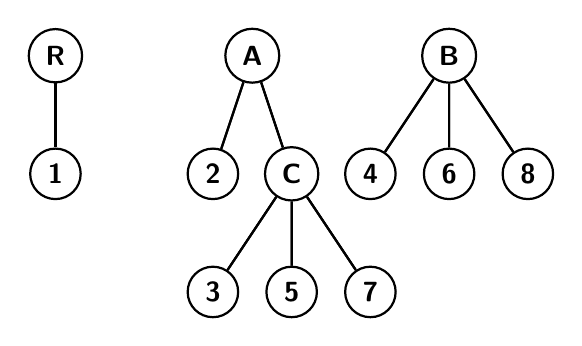
\begin{tikzpicture}[node distance=2.5cm,level distance=1.5cm,
                            level 1/.style={sibling distance=1cm},
                            level 2/.style={sibling distance=1cm},
                            thick,main node/.style={circle,draw,font=\sffamily\bfseries}]

        % Define vertices
        \node[main node] (R) {R}
            child {node[main node] (1) {1}};
        \node[main node] (A) [right of=R] {A}
            child {node[main node] (2) {2}}
            child {node[main node] (C) {C}
                child {node[main node] (3) {3}}
                child {node[main node] (5) {5}}
                child {node[main node] (7) {7}}
            };
        \node[main node] (B) [right of=A] {B}
            child {node[main node] (4) {4}}
            child {node[main node] (6) {6}}
            child {node[main node] (8) {8}};


        % Draw edges
        \path[every node/.style={font=\sffamily\small}]
            (R) edge (1)
            (A) edge (2)
            (A) edge (C)
            (B) edge (4)
            (B) edge (6)
            (B) edge (8)
            (C) edge (3)
            (C) edge (5)
            (C) edge (7);
        \end{tikzpicture}
        \caption{SCC Tree of Graph \ref{fig:graph1} after updates}
        \label{fig:scc_tree_graph_after_del}
    \end{subfigure}
    \caption{SCC Tree updates are propogated, deleting edge 4 to 1}
    \label{fig:scc_tree_after_update_propogation}
\end{figure}


\begin{figure}[H]
    \centering
    \begin{subfigure}{0.45\textwidth}
        \centering
        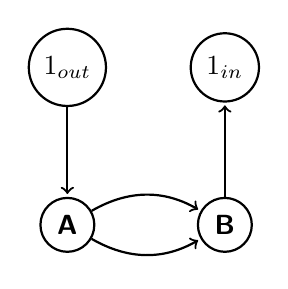
\begin{tikzpicture}[->,shorten >=1pt,auto,node distance=2cm,
            thick,main node/.style={circle,draw,font=\sffamily\bfseries}]

        % Define vertices
        \node[main node] (1) {$1_{in}$};
        \node[main node] (11) [left of=1] {$1_{out}$};
        \node[main node] (A) [below of=11] {A};
        \node[main node] (B) [below of=1] {B};
        

        % Draw edges
        \path[every node/.style={font=\sffamily\small}]
            (11) edge (A)
            (A) edge[bend left] (B)
            (A) edge[bend right] (B)
            (B) edge (1);

        \end{tikzpicture}
        \caption{Graph in SCC Tree Node R}
    \end{subfigure}
    \hfill
    \begin{subfigure}{0.45\textwidth}
        \centering
        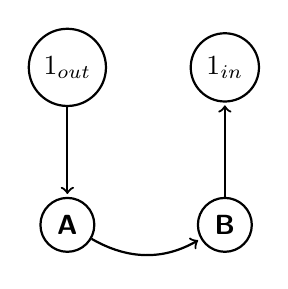
\begin{tikzpicture}[->,shorten >=1pt,auto,node distance=2cm,
            thick,main node/.style={circle,draw,font=\sffamily\bfseries}]

        % Define vertices
        \node[main node] (1) {$1_{in}$};
        \node[main node] (11) [left of=1] {$1_{out}$};
        \node[main node] (A) [below of=11] {A};
        \node[main node] (B) [below of=1] {B};
        

        % Draw edges
        \path[every node/.style={font=\sffamily\small}]
            (11) edge (A)
            (A) edge[bend right] (B)
            (B) edge (1);

        \end{tikzpicture}
        \caption{Graph after deleting edge 3 to 8}
        \label{fig:graph_after_dedge_3_to_8}
    \end{subfigure}
    \caption{Graph in SCC Tree Node R after deleting edge 3 to 8}
    \label{fig:tree_node_r_graph_after_dedge2}
\end{figure}
\subsubsection{Deleting Edge from an Internal Node}\label{Subsubsec: Deleting Edge from an Internal Node}

In this example, we consider the case when the deleted edge (u, v) belongs to an internal node of the SCC tree.
The edge (4, 8) is deleted from the graph held in \textsc{STN}(B), since the lowest common ancestor of 4 and 8 is B from the SCC tree in \figureref{\ref{fig:scc_tree_graph1}}.
We can see in \figureref{\ref{fig:tree_node_b_graph_after_dedge1}} that after removing the edge (4, 8) from the graph in \textsc{STN}(B), vertices 6 and 8 become unreachable from 4.


\begin{figure}[H]
    \centering
    \begin{subfigure}{0.45\textwidth}
        \centering
        \begin{tikzpicture}[->,shorten >=1pt,auto,node distance=2cm,
            thick,main node/.style={font=\sffamily\large\bfseries}]

        % Define vertices
        \node[main node] (4) {$4_{in}$};
        \node[main node] (44) [left of=1] {$4_{out}$};
        \node[main node] (6) [below of=1] {6};
        \node[main node] (8) [below of=11] {8};
        

        % Draw edges
        \path[every node/.style={font=\sffamily\small}]
            (44) edge (8)
            (8) edge (6)
            (6) edge (4);

        \end{tikzpicture}
        \caption{Graph in Tree Node B}
        \label{fig:tree_node_b_graph}
    \end{subfigure}
    \hfill
    \begin{subfigure}{0.45\textwidth}
        \centering
        \begin{tikzpicture}[->,shorten >=1pt,auto,node distance=2cm,
            thick,main node/.style={font=\sffamily\large\bfseries}]

        % Define vertices
        \node[main node] (4) {$4_{in}$};
        \node[main node] (44) [left of=1] {$4_{out}$};
        \node[main node] (6) [below of=1] {6};
        \node[main node] (8) [below of=11] {8};
        

        % Draw edges
        \path[every node/.style={font=\sffamily\small}]
            (8) edge (6)
            (6) edge (4);

        \end{tikzpicture}
        \caption{Graph after deleting edge 4 to 8}
        \label{fig:graph_after_dedge_4_to_8}
    \end{subfigure}
    \caption{Graph in Tree Node B after deleting edge 4 to 8}
    \label{fig:tree_node_b_graph_after_dedge1}
\end{figure}

Since, vertices 6 and 8 are unreachable from 4, we expose these vertices and the corresponding edges in \textsc{STN}(B) to its parent node R.
As shown in \figureref{\ref{fig:tree_node_r_graph_exposed1}}, the unreachable nodes 6 and 8 are exposed to the parent node R by adding edges (8,6), (6,4) from $B$ and
changing the edges (A,B), (B, $1_{in}$) in $R$ to (A,8), (4, $1_{in}$) respectively. The red line in \figureref{\ref{fig:tree_node_r_graph_exposed1}} shows the exposed graph
which was initially a part of $B$.

\begin{figure}[H]
    \centering
    \begin{subfigure}{0.45\textwidth}
        \centering
        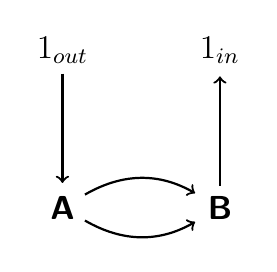
\begin{tikzpicture}[->,shorten >=1pt,auto,node distance=2cm,
            thick,main node/.style={font=\sffamily\large\bfseries}]

        % Define vertices
        \node[main node] (1) {$1_{in}$};
        \node[main node] (11) [left of=1] {$1_{out}$};
        \node[main node] (A) [below of=11] {A};
        \node[main node] (B) [below of=1] {B};
        

        % Draw edges
        \path[every node/.style={font=\sffamily\small}]
            (11) edge (A)
            (A) edge[bend left] (B)
            (A) edge[bend right] (B)
            (B) edge (1);

        \end{tikzpicture}
        \caption{Graph in SCC Tree Node R}
    \end{subfigure}
    \hfill
    \begin{subfigure}{0.45\textwidth}
        \centering
        \begin{tikzpicture}[->,shorten >=1pt,auto,node distance=2cm,
            thick,main node/.style={font=\sffamily\large\bfseries}]

        % Define vertices
        \node[main node] (1) {$1_{in}$};
        \node[main node] (11) [left of=1] {$1_{out}$};
        \node[main node] (A) [below left of=11] {A};
        \node[main node] (8) [below right of=A] {8};
        \node[main node] (6) [right of=8] {6};
        \node[main node] (4) [above right of=6] {4};
        

        % Draw edges
        \path[every node/.style={font=\sffamily\small}]
            (11) edge (A)
            (A) edge[bend left] (8)
            (A) edge[bend right] (8)
            (8) edge (6)
            (6) edge (4)
            (4) edge (1);

        \draw [red, rounded corners, dashed] ($(8) + (-0.5 , 0.5)$) -- ($(6) + (0,0.5)$) -- ($(4) + (-0.5, 0)$) -- ($(4) + (-0.5, 0.5)$) -- ($(4) + (0, 0.5)$) -- ($(4) + (0.5, 0.5)$) -- ($(4) + (0.5, 0)$) 
        -- ($(4) + (0.5, -0.25)$) -- ($(6) + (0.25, -0.5)$) -- ($(8) + (-0.5, -0.5)$) -- cycle;
        \end{tikzpicture}
        \caption{After Exposure}
        \label{fig:tree_node_r_graph_exposed1}
    \end{subfigure}
    \caption{Graph in SCC Tree Node R after unreachable nodes and its corresponding edges are exposed}
\end{figure}

We observe that every vertex in \figureref{\ref{fig:tree_node_r_graph_exposed1}} is reachable, thereby concluding the algorithm.
The above edge and vertex exposure process has a change in the SCC-tree, which is shown in \figureref{\ref{fig:scc_tree_after_update_propogation2}}.

\begin{figure}[H]
\centering
\begin{subfigure}{0.45\textwidth}
    \centering
    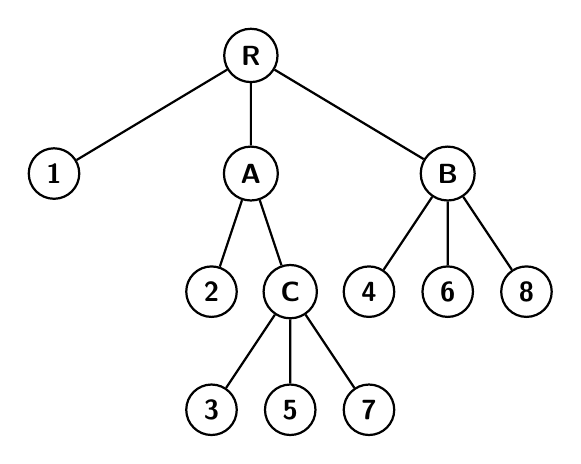
\begin{tikzpicture}[level distance=1.5cm,
                        level 1/.style={sibling distance=2.5cm},
                        level 2/.style={sibling distance=1cm},
                        thick,main node/.style={circle,draw,font=\sffamily\bfseries}]

    % Define vertices
    \node[main node] (R) {R}
        child {node[main node] (1) {1}}
        child {node[main node] (A) {A}
        child {node[main node] (2) {2}}
        child {node[main node] (C) {C}
            child {node[main node] (3) {3}}
            child {node[main node] (5) {5}}
            child {node[main node] (7) {7}}
        }
        }
        child {node[main node] (B) {B}
        child {node[main node] (4) {4}}
        child {node[main node] (6) {6}}
        child {node[main node] (8) {8}}
        };

    \end{tikzpicture}
    \caption{SCC Tree of Graph \ref{fig:graph1}}
\end{subfigure}
\hfill
\begin{subfigure}{0.45\textwidth}
    \centering
    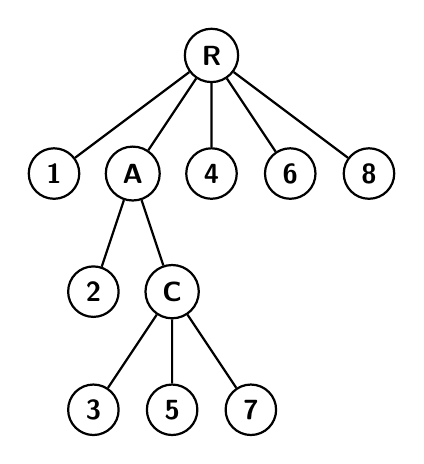
\begin{tikzpicture}[node distance=3cm,level distance=1.5cm,
                        level 1/.style={sibling distance=1cm},
                        level 2/.style={sibling distance=1cm},
                        thick,main node/.style={circle,draw,font=\sffamily\bfseries}]

    % Define vertices
    \node[main node] (R) {R}
        child {node[main node] (1) {1}}
        child {node[main node] (A) {A}
        child {node[main node] (2) {2}}
        child {node[main node] (C) {C}
        child {node[main node] (3) {3}}
        child {node[main node] (5) {5}}
        child {node[main node] (7) {7}}
        }
        }
        child {node[main node] (4) {4}}
        child {node[main node] (6) {6}}
        child {node[main node] (8) {8}}
        ;

    \end{tikzpicture}
    \caption{SCC Tree of Graph \ref{fig:graph1} after updates}
\end{subfigure}
\caption{Tree updates are propogated, deleting edge 4 to 8}
\label{fig:scc_tree_after_update_propogation2}
\end{figure}


\subsection{Incremental Maintaince of SCC Tree}\label{Subsec: Incremental Maintaince of SCC Tree}
\blindtext